% ====================================================================
% v7-01.tex — 흑연 음극 dQ/dV(ICA) 이론 Chapter 1 (v7, 독립 구현 01번)
%   척추 = v11_flowchart.md 의 N0→N9 진행 순서.
%   물리식 정본 = Anode_Fit_v11_final.py (706줄).
%   형식 기준 = graphite_ica_ch1_Opus_v5.tex (수식 주도).
%   build: xelatex 2-pass (kotex)
% ====================================================================
\documentclass[11pt,a4paper]{article}
\usepackage[margin=22mm]{geometry}
\usepackage{kotex}
\setmonofont{D2Coding}[Scale=MatchLowercase]
\usepackage{amsmath,amssymb,mathtools,bm}
\usepackage{booktabs,longtable,array}
\usepackage{enumitem}
\usepackage{amsthm}
\usepackage{hyperref}
\usepackage{fancyhdr}
\usepackage{lastpage}
\usepackage{setspace}
\usepackage{tikz}
\usetikzlibrary{positioning,arrows.meta}
\setstretch{1.12}
\setlength{\parskip}{0.45em}
\setlength{\parindent}{0pt}
\setlength{\headheight}{14pt}
\setlength{\emergencystretch}{2em}
\hypersetup{colorlinks=true, linkcolor=blue, urlcolor=blue, citecolor=blue,
  pdftitle={흑연 음극 dQ/dV 이론: Chapter 1 (v7-01)}}
\pagestyle{fancy}\fancyhf{}
\lhead{흑연 음극 $dQ/dV$ 이론 — Ch.1 (v7-01, 수식 주도)}\rhead{\thepage/\pageref{LastPage}}
\renewcommand{\headrulewidth}{0.4pt}

\newtheorem*{keybox}{핵심}
\newtheorem*{verifybox}{검산}
\newtheorem*{parambox}{피팅 초기값}

% 자주 쓰는 수식 단축 명령
\newcommand{\dd}{\mathrm{d}}
\newcommand{\app}{\mathrm{app}}
\newcommand{\eq}{\mathrm{eq}}
\newcommand{\eff}{\mathrm{eff}}
\newcommand{\bg}{\mathrm{bg}}
\newcommand{\cell}{\mathrm{cell}}
\newcommand{\hys}{\mathrm{hys}}
\newcommand{\dis}{\mathrm{dis}}
\newcommand{\chg}{\mathrm{chg}}
\newcommand{\peak}{\mathrm{peak}}

\renewcommand{\theequation}{1.\arabic{equation}}
\renewcommand{\thesection}{1.\arabic{section}}

\title{\textbf{\LARGE Chapter 1}\\[0.35em]
  \Large 흑연 음극 $dQ/dV$ 이론:\;코드 진행에서 피팅까지 — 수식 주도판 (v7-01)}
\author{}
\date{}

\makeatletter
\renewcommand*\l@section[2]{%
  \ifnum \c@tocdepth >\z@
    \addpenalty\@secpenalty
    \addvspace{1.0em \@plus\p@}%
    \setlength\@tempdima{2.3em}%
    \begingroup
      \parindent \z@ \rightskip \@pnumwidth
      \parfillskip -\@pnumwidth
      \leavevmode \bfseries
      \advance\leftskip\@tempdima
      \hskip -\leftskip
      #1\nobreak\hfil
      \nobreak\hb@xt@\@pnumwidth{\hss #2\kern-\p@\kern\p@}\par
    \endgroup
  \fi}
\renewcommand*\l@subsection{\@dottedtocline{2}{2.3em}{3.2em}}
\makeatother

\begin{document}
\maketitle

% ====================================================================
\section*{서론}
\addcontentsline{toc}{section}{서론}
% ====================================================================

흑연 음극의 \textbf{incremental capacity analysis}(ICA, $\dd Q/\dd V$)는 충방전
곡선 $Q(V)$ 를 전위로 미분해 staging 상전이마다 나타나는 peak 의 위치·너비·높이를
읽는다 \cite{bloom2005,dubarry2012}. 흑연은 stage $4\to3\to2\mathrm L\to2\to1$
전이를 거치며 \cite{dahn1991,ohzuku1993,funabiki1999}, 각 전이 전위 근방에서
$\dd Q/\dd V$ 가 치솟는 peak 하나를 남긴다.

관측된 peak 의 모양은 세 실험 인자 — \textbf{(a) 온도, (b) C-rate, (c) 충방전
방향} — 에 따라 변한다. 저온·고율일수록 꼬리가 길어지고, 충전과 방전에서 peak
가 서로 다른 전위에 나타나는 \emph{히스테리시스}가 생기며, 같은 전이가 C-rate
를 $0$ 으로 줄여도 사라지지 않는 열역학적 갈림을 보인다.

본 장은 \texttt{Anode\_Fit\_v11\_final.py} 클래스 \texttt{GraphiteAnodeDischargeDQDV}
의 계산 진행 N0→N9 를 절 순서로 삼아(Figure~\ref{fig:flowchart}), 각 단계에서
등장하는 물리식을 그 순서대로 유도한다. 코드 식별자는 v11\_final 과 1:1 로 대응하며,
이 문건만 보고 곡선 재현 코드를 작성할 수 있는 수준을 목표로 한다.

\begin{figure}[t]
\centering
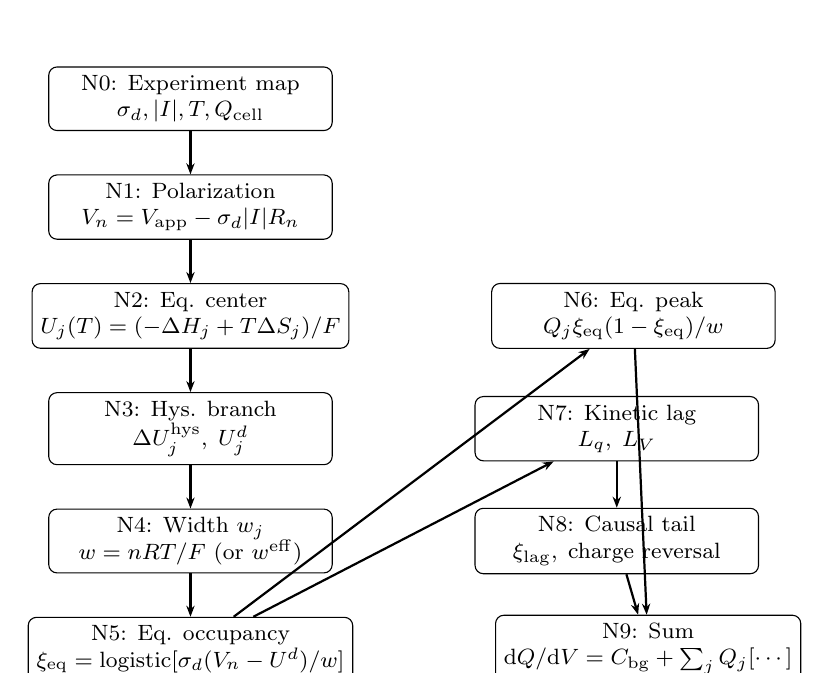
\begin{tikzpicture}[
  node distance=0.55cm and 1.8cm,
  box/.style={draw,rounded corners=3pt,minimum width=3.6cm,minimum height=7mm,
    inner sep=3pt,font=\footnotesize,align=center},
  arr/.style={-{Stealth[length=4pt]},thick}
]
\node[box] (n0) {N0: Experiment map\\$\sigma_d,|I|,T,Q_\cell$};
\node[box,below=of n0] (n1) {N1: Polarization\\$V_n = V_\app - \sigma_d|I|R_n$};
\node[box,below=of n1] (n2) {N2: Eq. center\\$U_j(T)=(-\Delta H_j+T\Delta S_j)/F$};
\node[box,below=of n2] (n3) {N3: Hys. branch\\$\Delta U_j^\hys,\;U_j^d$};
\node[box,below=of n3] (n4) {N4: Width $w_j$\\$w=nRT/F$ (or $w^\eff$)};
\node[box,below=of n4] (n5) {N5: Eq. occupancy\\$\xi_\eq=\mathrm{logistic}[\sigma_d(V_n-U^d)/w]$};
\node[box,right=of n2] (n6) {N6: Eq. peak\\$Q_j\xi_\eq(1-\xi_\eq)/w$};
\node[box,right=of n3] (n7) {N7: Kinetic lag\\$L_q,\;L_V$};
\node[box,right=of n4] (n8) {N8: Causal tail\\$\xi_\mathrm{lag},\;\text{charge reversal}$};
\node[box,right=of n5] (n9) {N9: Sum\\$\dd Q/\dd V = C_\bg+\sum_j Q_j[\cdots]$};
\draw[arr] (n0) -- (n1);
\draw[arr] (n1) -- (n2);
\draw[arr] (n2) -- (n3);
\draw[arr] (n3) -- (n4);
\draw[arr] (n4) -- (n5);
\draw[arr] (n5) -- (n6);
\draw[arr] (n5) -- (n7);
\draw[arr] (n6) -- (n9);
\draw[arr] (n7) -- (n8);
\draw[arr] (n8) -- (n9);
\end{tikzpicture}
\caption{v11\_final \texttt{dqdv()} 의 계산 진행(N0--N9). 각 노드가 본 장의 한 절에
대응한다. 방전 본론(N0--N7)을 먼저 전개하고, 히스 분기(N3)와 인과 기억
꼬리(N8)의 확장을 덧입힌다.}
\label{fig:flowchart}
\end{figure}

\tableofcontents
\newpage

% ====================================================================
\section{기호와 규약 (N0: 실험조건 매핑)}\label{sec:notation}
% ====================================================================

\texttt{curve(V\_app, direction, c\_rate, Q\_cell, T)} 가 최상위 진입점이다.
내부에서 방향 문자열을 방향 부호로, C-rate 를 전류 크기로 환산한 뒤
\texttt{dqdv(V\_app, T, I\_abs, Q\_cell, s)} 를 호출한다:
\begin{equation}
\sigma_d = \texttt{\_direction\_to\_sigma(direction)}\in\{+1,-1\},\qquad
|I| = \texttt{c\_rate}\times Q_\cell.
\label{eq:n0map}
\end{equation}
본 절은 이 매핑을 공식화하고, 이후 절에서 쓸 기호를 한 곳에 정의한다.

\subsection{부호 규약}

방전($\sigma_d=+1$): 전위 $V_n$ 이 상승하면서 탈리튬화(진행률 $\xi_j: 0\to1$).

충전($\sigma_d=-1$): 전위 $V_n$ 이 하강하면서 리튬화($\xi_j: 1\to0$).

\textbf{핵심 부호 사슬.} $\xi_\eq = \mathrm{logistic}[\sigma_d(V_n-U_j)/w_j]$ 이므로,
방전($\sigma_d=+1$)에서 $V_n\uparrow\Rightarrow\xi_\eq\uparrow$ (탈리튬화 진행), 충전에서는 반대.
$\dd\xi_\eq/\dd V_n = \sigma_d\,\xi_\eq(1-\xi_\eq)/w_j$ 는 \emph{방향 불변 양수} — 방전과
충전 모두 peak 기여가 양수다.

\begin{longtable}{p{0.14\textwidth} p{0.12\textwidth} p{0.66\textwidth}}
\toprule 기호 & 단위 & 의미 \\ \midrule \endhead
\multicolumn{3}{l}{\emph{--- 실험 입력(N0) ---}}\\
$V_\app$ & V & 측정 전위(인가 전위)\\
$\sigma_d$ & --- & 방향 부호: 방전 $+1$ / 충전 $-1$\\
$|I|$ & A (또는 C/s) & 전류 크기\\
$Q_\cell$ & C & 셀 용량; $q=\int|I|\,\dd t/Q_\cell$ 로 무차원화\\
$T$ & K & 절대 온도(스칼라 또는 배열 $T(V)$ 비등온)\\
\multicolumn{3}{l}{\emph{--- 분극(N1) ---}}\\
$V_n$ & V & 내부(열역학) 전위: $V_n=V_\app-\sigma_d|I|R_n$\\
$R_n$ & $\Omega$ & lumped 분극 저항\\
\multicolumn{3}{l}{\emph{--- 평형(N2--N5) ---}}\\
$j$ & --- & staging 전이 인덱스 ($j=1,\dots,N_p$, $N_p\approx3$--$4$)\\
$U_j(T)$ & V & 전이 $j$ 의 평형 중심 전위 (vs Li/Li$^+$)\\
$\Delta H_j,\Delta S_j$ & J/mol;\;J/(mol\,K) & 삽입 반응 엔탈피·엔트로피(\texttt{dH\_rxn, dS\_rxn})\\
$\Omega_j$ & J/mol & 정규용액 상호작용 에너지(\texttt{Omega})\\
$\gamma_j$ & --- & 히스 분기 축소 인자(\texttt{gamma}), $0\le\gamma_j\le1$\\
$h_\eta$ & --- & 부분 cycle 인자(\texttt{h\_eta}), 기본 $1.0$\\
$\Delta U_j^\hys$ & V & spinodal 상한 분기 gap\\
$U_j^d$ & V & 방향별 분기 중심 $=U_j+\tfrac12\sigma_d h_\eta\gamma_j\Delta U_j^\hys$\\
$n_j$ & --- & 폭 다중도(\texttt{n}; 없으면 $1$)\\
$w_j$ & V & 전이 폭: 이상 $nRT/F$, 유효 $w^\eff$\\
$\xi_{\eq,j}$ & --- & 평형 점유율(logistic)\\
$Q_j$ & C & 전이 $j$ 의 용량 가중(\texttt{Q})\\
$C_\bg$ & C/V & 배경 미분용량(\texttt{Cbg})\\
\multicolumn{3}{l}{\emph{--- 동역학(N7--N8) ---}}\\
$\Delta H_{a,j}$ & J/mol & 활성화 엔탈피(\texttt{dH\_a})\\
$\Delta S_{a,j}$ & J/(mol\,K) & 활성화 엔트로피(\texttt{dS\_a}, 기본 0)\\
$\chi$ & --- & 전달계수(\texttt{chi}; \texttt{x} 에서 상속)\\
$\chi_d$ & --- & 방향별 전달계수: 방전 $\chi$ / 충전 $1-\chi$\\
$\Delta H_{a,j}^\eff$ & J/mol & 유효 활성화 엔탈피 $=\Delta H_{a,j}-\chi_d\Omega_j$\\
$A_j$ & J/mol & 컷 affinity: $\min(z_\mathrm{cut}\cdot n_jRT,\;A_\mathrm{cap}RT)$\\
$L_{q,j}$ & --- & 용량축 지연 길이\\
$L_{V,j}$ & V & 전압축 지연 길이 $=|\dd V_n/\dd q|_{q_a}\cdot L_{q,j}$\\
$\xi_\mathrm{lag}$ & --- & 인과 기억 필터 출력\\
\multicolumn{3}{l}{\emph{--- 물리상수 ---}}\\
$R,F,k_B,h,N_A$ & --- & 기체상수, Faraday, Boltzmann, Planck, Avogadro\\
\bottomrule
\end{longtable}

% ====================================================================
\section{분극 보정 (N1)}\label{sec:polcorr}
% ====================================================================

측정 전위 $V_\app$ 는 내부 열역학 전위 $V_n$ 에 $IR$ 분극이 더해진 값이다.
정전류 실험에서 전하 보존 방정식의 해는 $V_n$ 이고, 관측되는 단자 전압이
$V_\app$ 이다. 두 전위의 관계는 방향 부호 $\sigma_d$ 를 명시하면:
\begin{equation}
\boxed{\;V_n = V_\app - \sigma_d\,|I|\,R_n\;.}
\label{eq:vn}
\end{equation}
방전($\sigma_d=+1$): 산화 방향이라 전류가 흐를 때 내부 전위가 단자 전압보다 낮다
($V_n < V_\app$). 충전($\sigma_d=-1$): 내부 전위가 단자 전압보다 높다
($V_n > V_\app$). 이후 절의 모든 물리식은 $V_n$(열역학 전위)을 독립 변수로 쓴다.

\begin{figure}[t]
\centering
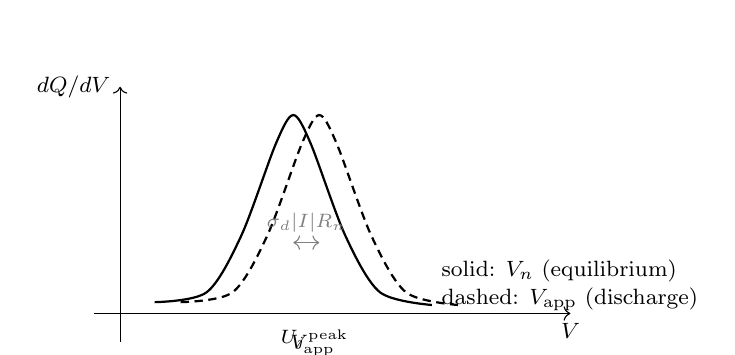
\begin{tikzpicture}[x=2.2cm,y=1.8cm]
% 축
\draw[->] (-0.15,0) -- (2.6,0) node[below] {\footnotesize $V$};
\draw[->] (0,-0.2) -- (0,1.6) node[left] {\footnotesize $dQ/dV$};
% 평형 곡선 (실선)
\draw[thick] plot[smooth] coordinates
  {(0.2,0.08)(0.5,0.15)(0.7,0.55)(0.9,1.2)(1.0,1.4)(1.1,1.2)(1.3,0.55)(1.5,0.15)(1.8,0.06)};
% 방전 곡선 (파선, 오른쪽 이동)
\draw[thick,densely dashed] plot[smooth] coordinates
  {(0.35,0.08)(0.65,0.15)(0.85,0.55)(1.05,1.2)(1.15,1.4)(1.25,1.2)(1.45,0.55)(1.65,0.15)(1.95,0.06)};
% 화살표 및 라벨
\draw[<->,gray] (1.0,0.5) -- (1.15,0.5) node[pos=0.5,above] {\scriptsize $\sigma_d|I|R_n$};
\node[below] at (1.0,-0.05) {\scriptsize $U_j$};
\node[below] at (1.15,-0.05) {\scriptsize $V_\app^\peak$};
\node[right] at (1.8,0.3) {\footnotesize solid: $V_n$ (equilibrium)};
\node[right] at (1.8,0.1) {\footnotesize dashed: $V_\app$ (discharge)};
\end{tikzpicture}
\caption{분극에 의한 peak 이동. 방전($\sigma_d=+1$) 시 측정 전위가 내부 전위보다
$|I|R_n$ 만큼 오른쪽(고전위 쪽)으로 이동한다. 식~\eqref{eq:vn} 의 보정으로
$V_n$ 을 복원한 뒤 이후 물리식을 적용한다.}
\label{fig:polshift}
\end{figure}

분극에 의한 peak 이동이 Figure~\ref{fig:polshift} 에 도시되어 있다.
$R_n$ 측정은 전류 차단 직후 도약 전압에서 직독하고(\S\ref{sec:fitting} S2), 이 값을
식~\eqref{eq:vn} 에 넣어 전 데이터셋에서 $V_n$ 을 복원한다.

다음 절부터는 $V_n$ 을 격자로 작업한다. 코드에서는 \texttt{dqdv()} L412 가
\texttt{V\_n = V\_in - sigma\_d * I\_abs * self.Rn} 으로 구현한다.

% ====================================================================
\section{평형 중심 전위 (N2)}\label{sec:eqcenter}
% ====================================================================

식~\eqref{eq:vn} 의 $V_n$ 이 만들어지면, 각 staging 전이 $j$ 에 대해 열역학
평형 중심 전위 $U_j(T)$ 를 계산한다. 이 양은 삽입 반응의 Gibbs 자유에너지
변화에서 직접 유도된다.

\subsection{열역학 유도: $\Delta G = -FU$}

삽입 반응 $\mathrm{Li}^++e^-+[\;]\rightleftharpoons\mathrm{Li}_{(\text{흑연})}$ 에서
1전자 과정($z=1$)이라 전기화학적 평형 조건은 $\Delta G_j = -FU_j$ 다.
$\Delta G_j = \Delta H_j - T\Delta S_j$ 를 넣으면:
\begin{equation}
\boxed{\;U_j(T) = \frac{-\Delta H_j + T\,\Delta S_j}{F}\;.}
\label{eq:Uj}
\end{equation}
$\Delta H_j < 0$(발열 삽입)이면 $U_j > 0$ 이 되고 리튬이 흑연에 자발 삽입한다.
온도 의존성은 Gibbs 항등식 $\partial\Delta G/\partial T = -\Delta S$ 로:
\begin{equation}
\frac{\partial U_j}{\partial T} = \frac{\Delta S_j}{F}.
\label{eq:dUdT}
\end{equation}
$|\Delta S_j|\sim$ 수 J/(mol\,K) 이므로 $|\partial U_j/\partial T|\approx0.01$--$0.1$ mV/K.
$30$ K 창에서 $0.3$--$3$ mV — 다온도 피팅에서 온도마다 $U_j(T)$ 를 따로 읽어야 하는
이유다.

코드: \texttt{func\_U\_j(T, dH\_rxn, dS\_rxn)} (L68) $= (-\Delta H+T\Delta S)/F$,
또는 전이 딕셔너리에 \texttt{'U'} 직접 지정 시 우선.

\begin{verifybox}
\textbf{수치 예.} stage $2\to1$ 전이: $\Delta H=-13.0$ kJ/mol, $\Delta S=-16$ J/(mol\,K)
(\texttt{GRAPHITE\_STAGING\_LIT} 마지막 항목). $T=298.15$ K 에서
$U=[-(-13000)+298.15\times(-16)]/96485=(13000-4770.4)/96485\approx0.085$ V — 코드 \texttt{'U': 0.085} 와 정합.
\end{verifybox}

\subsection{온도 배열 지원}

코드 L438 에서 $T$ 가 배열(\texttt{T\_work})이면 \texttt{func\_U\_j(T\_work, dH\_rxn, dS\_rxn)}
으로 $U_j$ 도 배열이 된다. 비등온 조건(주행 중 온도 분포)을 자연스럽게 처리한다.

이 절이 제공하는 $U_j(T)$ 를 다음 절(N3)의 히스 분기 계산에서 기준값으로 쓴다.

% ====================================================================
\section{히스테리시스 분기 (N3)}\label{sec:hys}
% ====================================================================

\subsection{정규용액 모형과 상분리}

격자기체 모형에서 점유 이웃 쌍의 상호작용 에너지를 평균장으로 쓰면, Li 자리
1몰당 자유에너지는:
\begin{equation}
g_j(\xi) = g_j^0 + RT\bigl[\xi\ln\xi + (1-\xi)\ln(1-\xi)\bigr] + \Omega_j\,\xi(1-\xi).
\label{eq:gxi}
\end{equation}
엔트로피 항(아래 볼록)과 상호작용 항 $\Omega_j\xi(1-\xi)$(위로 올림)이 경쟁한다.
$\Omega_j > 2RT$ 이면 가운데가 언덕인 이중 우물 — 한 전위에 여러 $\xi$ 가 대응하는
상분리 영역이 생긴다(임계온도 $T_{c,j}=\Omega_j/2R$). 식~\eqref{eq:gxi} 를 두 번 미분하면:
\begin{equation}
g_j''(\xi) = \frac{RT}{\xi(1-\xi)} - 2\Omega_j,
\end{equation}
$g_j''=0$ 의 두 근이 \textbf{spinodal} 좌표다:
\begin{equation}
\xi_{s,j}^\pm = \tfrac12 \pm \tfrac12\,u_j,\qquad
u_j \equiv \sqrt{1-\frac{2RT}{\Omega_j}}\quad(\Omega_j > 2RT).
\label{eq:spinodal}
\end{equation}

\subsection{분기 gap 의 닫힌 식}

비단조 평형 전위 곡선에서 방전(탈리튬화, $\xi\uparrow$)은 spinodal 대값
$\xi_{s,j}^+ = \tfrac12+\tfrac12 u_j$ 까지, 충전(리튬화, $\xi\downarrow$)은 소값
$\xi_{s,j}^- = \tfrac12-\tfrac12 u_j$ 까지 과주행한다.
두 극값의 전위 차가 spinodal 상한 분기 gap 이다.
$\xi_{s,j}^\pm$ 를 평형 전위 식에 대입해 빼면:
\begin{equation}
\boxed{\;\Delta U_j^\hys =
  \frac{2}{F}\bigl[\Omega_j\,u_j - 2RT\,\mathrm{artanh}\,u_j\bigr],\qquad
  u_j = \sqrt{1-\frac{2RT}{\Omega_j}}\;.}
\label{eq:dUhys}
\end{equation}
극한: $\Omega_j \le 2RT$ 이면 $u_j$ 가 허수 $\Rightarrow \Delta U_j^\hys = 0$. 코드:
\texttt{func\_dU\_hys(T, Omega)} (L123).

임계 근방 Taylor 전개($u_j\to0$): $\mathrm{artanh}\,u \approx u + u^3/3 + \cdots$
를 식~\eqref{eq:dUhys} 에 넣으면 $\Delta U_j^\hys \propto u_j^3 \propto (T_{c,j}-T)^{3/2}$.
절편의 온도 의존이 이 멱을 따르는지 확인하면 $\Omega_j$ 가 식별된다.

\subsection{분기 중심}

실측 분기는 spinodal 상한보다 안쪽에서 열리므로(핵생성 속도·다입자 mosaic 효과)
현상학적 축소 인자 $\gamma_j\in[0,1]$ 과 부분 cycle 인자 $h_\eta$ 를 도입한다:
\begin{equation}
\boxed{\;U_j^d = U_j + \tfrac12\,\sigma_d\,h_\eta\,\gamma_j\,\Delta U_j^\hys\;.}
\label{eq:Ubranch}
\end{equation}
방전($\sigma_d=+1$): $U_j^d = U_j + \tfrac12\gamma_j\Delta U_j^\hys > U_j$ (고전위 쪽).
충전($\sigma_d=-1$): $U_j^d = U_j - \tfrac12\gamma_j\Delta U_j^\hys < U_j$ (저전위 쪽).
$\gamma_j=0$ 이면 분기 없음, $\gamma_j=1$ 이면 spinodal 상한. 코드:
\texttt{func\_U\_branch(T, U\_j, Omega, gamma, sigma\_d, h\_eta)} (L133).

$\gamma_j=0$ 이거나 $\Omega_j=0$ 이면 $U_j^d = U_j$ — 방향 불변 평형 peak 로 환원.

이제 다음 절(N4, N5)에서 분기 중심 $U_j^d$ 를 중심으로 폭과 점유율을 정한다.

% ====================================================================
\section{전이 폭과 평형 점유율 (N4, N5)}\label{sec:eqocc}
% ====================================================================

\subsection{통계역학에서 logistic 까지}

분기 중심 $U_j^d$ 가 정해지면, 그 중심 주변 전위에서의 평형 점유율 $\xi_\eq$ 를
logistic 형태로 유도한다. 출발점은 격자기체 화학퍼텐셜과 전기화학 평형 조건의 결합이다.

격자기체 화학퍼텐셜의 로그 항 $RT\ln[\xi/(1-\xi)]$ 와 전기화학 평형 조건
$\mu = -F(V_n - U_j)$ 를 연결하면($\Omega_j=0$ 이상 극한):
\begin{equation}
RT\ln\frac{\xi_\eq}{1-\xi_\eq} = F\,\sigma_d\,(V_n - U_j^d),
\end{equation}
양변을 $\exp$ 해 $\xi_\eq$ 에 대해 풀면:
\begin{equation}
\xi_\eq = \frac{e^{\sigma_d(V_n-U_j^d)/w_j}}{1+e^{\sigma_d(V_n-U_j^d)/w_j}}
= \frac{1}{1+e^{-\sigma_d(V_n-U_j^d)/w_j}},\qquad
w_j \equiv \frac{n_j RT}{F}.
\label{eq:ksi_eq_deriv}
\end{equation}
이것이 logistic 함수다. 코드:
\texttt{func\_ksi\_eq(T, V\_n, U, n, s)} (L84):
\begin{equation}
\boxed{\;\xi_{\eq,j}(V_n, T) = \mathrm{logistic}\!\left[\frac{\sigma_d(V_n - U_j^d)}{w_j}\right],\qquad
w_j = \frac{n_j RT}{F}\;.}
\label{eq:ksi_eq}
\end{equation}

\subsection{폭 척도}

이상 극한($\Omega_j=0$): $w_j = n_j RT/F$, $25^\circ$C 에서 $25.7$ mV ($n_j=1$).
코드: \texttt{func\_w(T, n)} (L64).

유효 폭(옵션 \texttt{use\_w\_eff=True}): 상호작용이 등온선을 좁히므로 중심 기울기
$\dd V_n/\dd\xi|_{1/2}$ 에서 등가 폭을 읽으면:
\begin{equation}
w_j^\eff = \frac{RT}{F}\left(1 - \frac{\Omega_j}{2RT}\right)
\quad(\Omega_j \le 2RT).
\label{eq:weff}
\end{equation}
$\Omega_j \to 2RT$ 에서 $w^\eff \to 0$, $\Omega_j > 2RT$ 이면 등온선이 비단조가 되어
단일 폭 근사가 무효다. 코드: \texttt{func\_w\_eff(T, Omega, floor\_frac)} (L141).

\begin{figure}[t]
\centering
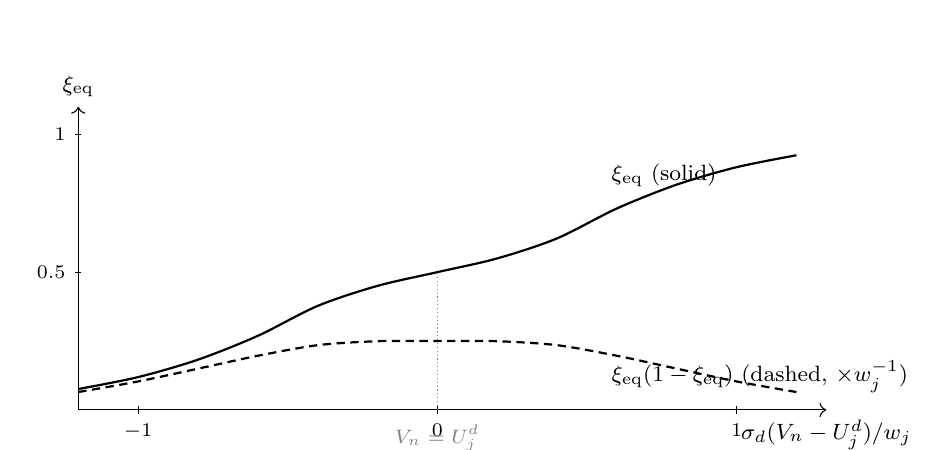
\begin{tikzpicture}[x=3.8cm,y=3.5cm]
\draw[->] (-1.2,0) -- (1.3,0) node[below] {\footnotesize $\sigma_d(V_n-U_j^d)/w_j$};
\draw[->] (-1.2,0) -- (-1.2,1.1) node[above] {\footnotesize $\xi_\eq$};
\foreach \x in {-1,0,1} {\draw (\x,0.015) -- (\x,-0.015) node[below] {\scriptsize $\x$};}
\foreach \y in {0.5,1} {\draw (-1.19,\y) -- (-1.21,\y) node[left] {\scriptsize $\y$};}
% logistic curve
\draw[thick] plot[smooth] coordinates
{(-1.2,0.0759)(-1.0,0.1192)(-0.8,0.1824)(-0.6,0.2689)(-0.4,0.3775)
(-0.2,0.4502)(0,0.5)(0.2,0.5498)(0.4,0.6225)(0.6,0.7311)
(0.8,0.8176)(1.0,0.8808)(1.2,0.9241)};
% derivative bell curve (scaled for display)
\draw[thick,densely dashed] plot[smooth] coordinates
{(-1.2,0.065)(-1.0,0.1034)(-0.8,0.1498)(-0.6,0.1966)(-0.4,0.2350)
(-0.2,0.2494)(0,0.25)(0.2,0.2494)(0.4,0.2350)(0.6,0.1966)
(0.8,0.1498)(1.0,0.1034)(1.2,0.065)};
\draw[gray,densely dotted] (0,0) -- (0,0.5);
\node[below,gray] at (0,-0.02) {\scriptsize $V_n=U_j^d$};
\node[right] at (0.55,0.85) {\footnotesize $\xi_\eq$ (solid)};
\node[right] at (0.55,0.12) {\footnotesize $\xi_\eq(1-\xi_\eq)$ (dashed, $\times w_j^{-1}$)};
\end{tikzpicture}
\caption{logistic 등온선~\eqref{eq:ksi_eq}(실선)과 그 미분 $\xi_\eq(1-\xi_\eq)$(파선).
미분이 $V_n=U_j^d$ 에서 최대 $1/4$ — 평형 peak 의 모양이다(\S\ref{sec:eqpeak}).
방향 부호 $\sigma_d$ 는 logistic 인수에만 들어가므로 미분의 \emph{부호는 방향 불변}.}
\label{fig:logistic}
\end{figure}

\subsection{부호 검산}

logistic 등온선과 그 미분의 모양은 Figure~\ref{fig:logistic} 에 도시되어 있다.
$\sigma_d=+1$(방전), $V_n \gg U_j^d$: $\xi_\eq \to 1$ (완전 탈리튬화).
$V_n = U_j^d$: $\xi_\eq = 1/2$ (전이 중심).
$V_n \ll U_j^d$: $\xi_\eq \to 0$ (미탈리튬화).
$\sigma_d=-1$(충전)에서는 $V_n\downarrow$ 가 $\xi_\eq\downarrow$(리튬화 진행) — 식~\eqref{eq:ksi_eq}
부호 사슬 전건 정합.

% ====================================================================
\section{평형 peak 기준선 (N6)}\label{sec:eqpeak}
% ====================================================================

$|I|\to0$ 한계에서 전이의 기여는 logistic 의 전위 미분이다. 식~\eqref{eq:ksi_eq}
를 $z \equiv \sigma_d(V_n-U_j^d)/w_j$ 로 치환해 미분하면:
\begin{equation}
\frac{\dd\xi_\eq}{\dd z} = \xi_\eq(1-\xi_\eq),
\end{equation}
연쇄율 $\dd z/\dd V_n = \sigma_d/w_j$ 를 곱하면:
\begin{equation}
\frac{\dd\xi_{\eq,j}}{\dd V_n} = \frac{\sigma_d\,\xi_{\eq,j}(1-\xi_{\eq,j})}{w_j}.
\label{eq:dxidV}
\end{equation}
전하 보존 미분 $\dd Q/\dd V_n = C_\bg + \sum_j Q_j\,\dd\xi_j/\dd V_n$ 에 대입하면:
\begin{equation}
\boxed{\;\left.\frac{\dd Q}{\dd V_n}\right|_\eq
= C_\bg(V_n,T)
+ \sum_{j=1}^{N_p} Q_j\,\frac{\xi_{\eq,j}(1-\xi_{\eq,j})}{w_j}\;.}
\label{eq:eqpeak}
\end{equation}
분모에 $w_j$ 가 있으므로 $\sigma_d$ 는 약분되어 \textbf{방향 불변 양수}.
코드 L468 에서 \texttt{peak\_shape = ksi\_eq * (1 - ksi\_eq) / w} 가 이 식이다.

Peak 의 세 특성:
\begin{align}
V_\peak &= U_j^d(T), \label{eq:peakpos}\\
\left.\frac{\dd Q}{\dd V_n}\right|_{\max}^\mathrm{net} &= \frac{Q_j}{4w_j}\quad\text{($\xi_\eq=1/2$ 에서 $\xi(1-\xi)=1/4$)},\label{eq:peakheight}\\
\int\!\left(\frac{\dd Q}{\dd V_n} - C_\bg\right)\dd V_n &= Q_j.\label{eq:peakarea}
\end{align}
저온일수록 $w_j\propto T$ 가 작아 peak 가 좁고 높다(면적 $Q_j$ 보존).

코드 \texttt{equilibrium(V\_n, T)} (L354)는 식~\eqref{eq:eqpeak} 의 직접 구현이며,
$|I|\to0$ 한계 기준선을 생성한다.

% ====================================================================
\section{동역학 지연 길이 (N7)}\label{sec:kinlag}
% ====================================================================

$|I|>0$ 이면 반응 속도 $k_j$ 의 공급이 전류 요구를 따라가지 못해 평형 점유율
$\xi_{\eq,j}$ 와 실제 점유율 $\xi_j$ 사이에 지연 $r_j = \xi_{\eq,j} - \xi_j$ 가
생긴다. 이 절이 지연의 특성 길이를 닫는다.

\subsection{Eyring 속도식과 보편 시도 빈도}

전이상태 이론에서 장벽 $\Delta G_a$ 를 넘을 확률 $\propto e^{-\Delta G_a/RT}$ 이고,
보편 시도 빈도 $k_0 = k_BT/h$ 를 곱하면:
\begin{equation}
k = k_0\,e^{-\Delta G_a/RT},\qquad k_0=\frac{k_BT}{h},\qquad
\Delta G_a = \Delta H_a - T\Delta S_a.
\label{eq:eyring}
\end{equation}

\subsection{방향별 장벽 — Butler--Volmer 형}

구동력(affinity) $A_j = \min(z_\mathrm{cut}\,n_jRT,\;A_\mathrm{cap}RT)$
(코드: \texttt{\_resolve\_lag\_length} L335; 기본값 $z_\mathrm{cut}=4.357$,
$A_\mathrm{cap}=4.0$)에서 정방향 장벽이 $\chi_dA_j$ 만큼 낮아진다. 역방향 몫 $(1+e^{-A_j/RT})$ 까지 포함한 완화 속도 보편형:
\begin{equation}
k_j = k_0\,e^{-(\Delta G_{a,j}-\chi_dA_j)/RT}\bigl(1+e^{-A_j/RT}\bigr).
\label{eq:kuniv}
\end{equation}
$A_j \gtrsim 3RT$ 이면 역방향 몫 $\approx 5\%$ 로 작아 $k_j \simeq r_j^+$(forward 극한).

\subsection{방향별 전달계수 $\chi_d$}

정방향(탈리튬화, 방전 깊은 꼬리 $\xi\to1$)과 역방향(리튬화, 충전 깊은 꼬리 $\xi\to0$)
의 전이상태 위치가 다르다. 자세히 balance($r^+/r^- = e^{A_j/RT}$)가 강제하는
\textbf{합-1 규칙} $\chi + \chi' = 1$ 에서, 방전·충전 전달계수:
\begin{equation}
\chi_d = \begin{cases} \chi & \text{방전}\ (\sigma_d=+1) \\ 1-\chi & \text{충전}\ (\sigma_d=-1) \end{cases}.
\label{eq:chid}
\end{equation}
코드: \texttt{func\_chi\_d(chi, sigma\_d)} (L155), \texttt{\_chi\_d(sigma\_d)} (L291).

\subsection{유효 활성화 엔탈피}

깊은 꼬리($\xi_j\to1$, 방전)에서 상호작용 항 $\Omega_j$ 가 장벽에 상수 몫으로
흡수된다:
\begin{equation}
\Delta H_{a,j}^\eff = \Delta H_{a,j} - \chi_d\,\Omega_j.
\label{eq:dHeff}
\end{equation}
코드: \texttt{func\_dH\_a\_eff(dH\_a, Omega, chi\_d)} (L149). 충전 깊은 꼬리
($\xi\to0$, $\chi_d=1-\chi$)에서도 같은 구조로 $+\Omega_j$ 가 흡수 — 방향별
$\chi_d$ 가 자동 처리한다.

\subsection{용량축 지연 길이 $L_{q,j}$}

정전류 방전에서 $\dd q/\dd t = |I|/Q_\cell$ 이고, 운동방정식
$\dd\xi_j/\dd t = k_j(\xi_{\eq,j}-\xi_j)$ 를 $q$ 축으로 옮기면 지연 $r_j$ 는:
\begin{equation}
\frac{\dd r_j}{\dd q} = \frac{\dd\xi_{\eq,j}}{\dd q} - \frac{r_j}{L_{q,j}},\qquad
L_{q,j} \equiv \frac{|I|}{Q_\cell\,k_j}.
\label{eq:relaxq}
\end{equation}
식~\eqref{eq:eyring}·\eqref{eq:kuniv} 를 $k_j$ 에 넣으면:
\begin{equation}
\boxed{\;L_{q,j} = \frac{|I|\,h}{Q_\cell k_BT}\,
  \frac{e^{(\Delta H_{a,j}^\eff - \chi_d A_j)/RT}}{1 + e^{-A_j/RT}}\;.}
\label{eq:Lq}
\end{equation}
코드: \texttt{func\_L\_q(T, I, Q\_cell, dH\_a, dS\_a, x, A)} (L90).

로그 형태($-T\Delta S_a$ 는 절편에 흡수):
\begin{equation}
\ln L_{q,j} = \ln\frac{T_*}{T} + \frac{\Delta H_{a,j}^\eff - \chi_d A_j}{RT} + b_j,\qquad
T_* \equiv \frac{|I|\,h}{Q_\cell k_B}.
\label{eq:lnLq}
\end{equation}
$b_j = -\Delta S_{a,j}/R + \ln(1+e^{-A_j/RT})$ 는 온도 약의존 절편 — 다온도 피팅에서
$\Delta H_a^\eff$ 를 기울기에서, $b_j$ 를 절편에서 읽는다.

전압축 지연 길이:
\begin{equation}
L_{V,j} = \left|\frac{\dd V_n}{\dd q}\right|_{q_a}\!\! L_{q,j}.
\label{eq:LV}
\end{equation}
코드: \texttt{\_resolve\_lag\_length()} (L307) → L351.

\subsection{전위 의존: $V\uparrow\Rightarrow L\downarrow$}

$A_j = sF(V_n - U_j)$ 가 깊어질수록($V_n \uparrow$, 방전에서) 장벽이 낮아져
$k_j$ 증가 → $L_{q,j}$ 감소. 로그 미분:
\begin{equation}
\frac{\partial\ln L_{q,j}}{\partial V_n} \approx -\frac{\chi_d\,F}{RT} \le 0.
\label{eq:dLdV}
\end{equation}
구동이 깊을수록 꼬리가 짧아진다.

이 절이 계산한 $L_{V,j}$ 를 다음 절(N8)의 인과 기억 필터에 넘긴다.

% ====================================================================
\section{인과 기억 꼬리 (N8)}\label{sec:tail}
% ====================================================================

\subsection{지수 기억 합성곱의 일반해}

식~\eqref{eq:relaxq} 는 1계 선형 ODE 라 적분인자 $e^{q/L_{q,j}}$ 로 닫힌 해를
갖는다. 초기 지연 $r_j(q_0)=0$ 조건에서:
\begin{equation}
\boxed{\;r_j(q) = \int_{q_0}^q e^{-(q-q')/L_{q,j}}\,\frac{\dd\xi_{\eq,j}}{\dd q'}\,\dd q'\;.}
\label{eq:memory}
\end{equation}
지연은 ``과거 평형 목표 변화율을 지수 커널로 가중한 기억''의 합성곱이다.
커널 길이 $L_{q,j}$ 만큼의 최근 과거만 기억한다.

수치 구현은 재귀 지수 이동 평균(IIR 저역 필터):
\begin{equation}
\xi_\mathrm{lag}[i] = \alpha\,\xi_\mathrm{lag}[i-1] + (1-\alpha)\,\xi_\eq[i],\qquad
\alpha = e^{-\Delta V/L_{V,j}}
\label{eq:iir}
\end{equation}
($\Delta V$ = 격자 간격). 코드: \texttt{\_causal\_lowpass(source\_signal, grid\_step, lag\_length)} (L100),
\texttt{scipy.signal.lfilter} 를 쓰거나 순환 fallback.

\subsection{peak\_shape 와 평형 peak 로의 환원}

지연 필터 결과를 이용해 각 전이의 dQ/dV 기여 모양을 계산한다:
\begin{equation}
\text{peak\_shape}_j = \frac{\xi_{\eq,j} - \xi_{\mathrm{lag},j}}{L_{V,j}}.
\label{eq:peakshape}
\end{equation}
$L_{V,j}$ 가 충분히 작으면(정확히는 \texttt{min\_lag\_grid\_steps} $\times$ \texttt{grid\_step}
미만) 필터를 건너뛰고 평형 peak 를 직접 쓴다:
\begin{equation}
\text{peak\_shape}_j = \frac{\xi_{\eq,j}(1-\xi_{\eq,j})}{w_j}\quad (L_{V,j} \to 0 \text{ 한계}).
\label{eq:eqrecover}
\end{equation}
코드 L466--L468 의 분기가 이를 구현한다.

\subsection{★ 충전 격자 역전}

인과 기억 필터는 ``진행 방향의 과거'' 를 기억한다.
방전($\sigma_d=+1$): $V_n$ 이 상승하므로 격자 오름차순 그대로 필터.
충전($\sigma_d=-1$): $V_n$ 이 하강하므로 격자를 \emph{뒤집어} 필터 후 다시 되돌린다:
\begin{equation}
\xi_\mathrm{lag} = \texttt{\_causal\_lowpass}(\xi_\eq[::-1], \Delta V, L_{V,j})[::-1].
\label{eq:reverse}
\end{equation}
이 처리가 없으면 충전에서 꼬리가 반대 방향(물리적으로 불가능한 방향)으로 생긴다.
코드 L474--L477:
\begin{verbatim}
if sigma_d >= 0:
    occ_lagged = _causal_lowpass(ksi_arr, grid_step, lag_len_V)
else:
    occ_lagged = _causal_lowpass(ksi_arr[::-1], grid_step, lag_len_V)[::-1]
\end{verbatim}
격자 역전 결과: 충전 dQ/dV 는 방전의 거울상이 되어 \textbf{양수를 유지}한다
(부호 사슬 체크리스트 항목 7 충족). 동역학 꼬리의 시각적 모양은
Figure~\ref{fig:tail} 에 도시되어 있다.

\begin{figure}[t]
\centering
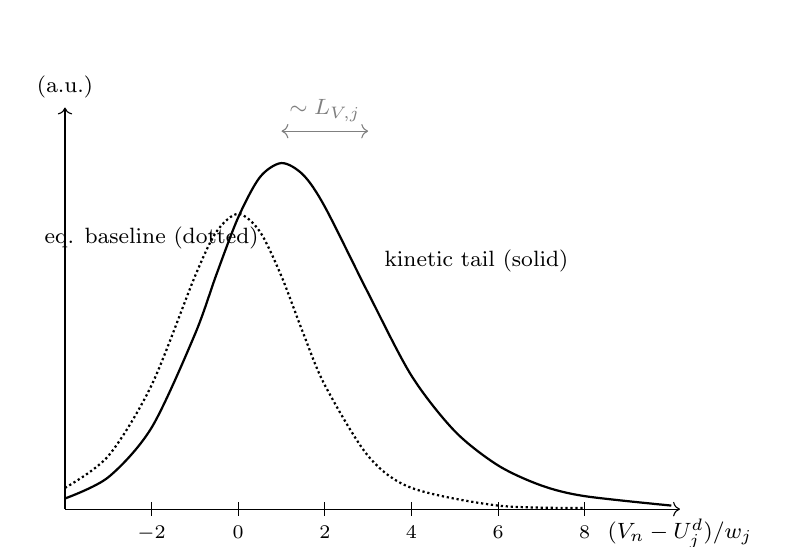
\begin{tikzpicture}[x=0.55cm,y=15cm]
\draw[->](-4,0) -- (10.2,0) node[below] {\footnotesize $(V_n - U_j^d)/w_j$};
\foreach \x in {-2,0,2,4,6,8} {\draw (\x,0.006) -- (\x,-0.006) node[below] {\scriptsize $\x$};}
\draw[->](-4,0) -- (-4,0.34) node[above] {\footnotesize (a.u.)};
% equilibrium bell
\draw[thick,densely dotted] plot[smooth] coordinates
{(-4,0.018)(-3,0.045)(-2,0.105)(-1,0.197)(-0.5,0.235)(0,0.25)(0.5,0.235)
(1,0.197)(1.5,0.149)(2,0.105)(3,0.045)(4,0.018)(6,0.003)(8,0.001)};
% kinetic peak (shifted, with tail)
\draw[thick] plot[smooth] coordinates
{(-4,0.009)(-3,0.027)(-2,0.069)(-1,0.148)(-0.5,0.199)(0,0.247)
(0.5,0.281)(1,0.293)(1.5,0.283)(2,0.256)(3,0.183)(4,0.113)(5,0.066)
(6,0.037)(7,0.020)(8,0.011)(10,0.003)};
\node at (-2,0.23) {\footnotesize eq. baseline (dotted)};
\node at (5.5,0.21) {\footnotesize kinetic tail (solid)};
\draw[<->,gray](1,0.32) -- (3,0.32) node[pos=0.5,above] {\footnotesize $\sim L_{V,j}$};
\end{tikzpicture}
\caption{동역학 꼬리의 발생. 점선: 평형 기준선 $\xi_\eq(1-\xi_\eq)/w_j$.
실선: 인과 기억 필터 후 \texttt{peak\_shape}~\eqref{eq:peakshape}.
$L_{V,j}$ 가 클수록 정점이 늦게 나타나고 꼬리가 길어진다.
두 곡선의 면적 합 $= Q_j$ 로 보존된다.}
\label{fig:tail}
\end{figure}

% ====================================================================
\section{전이 합산과 최종 dQ/dV (N9)}\label{sec:total}
% ====================================================================

전 전이의 기여를 배경에 선형으로 더한다:
\begin{equation}
\boxed{\;\frac{\dd Q}{\dd V_n}
= C_\bg(V_n,T)
+ \sum_{j=1}^{N_p} Q_j \cdot \text{peak\_shape}_j\;.}
\label{eq:total}
\end{equation}
코드 L481: \texttt{dqdv\_work += tr['Q'] * peak\_shape}.

$L_{V,j}$ 가 작은 전이(저율 또는 동역학 키 미지정)는 peak\_shape = 평형 bell, 큰
전이는 인과 기억 꼬리 형태. 두 경우 모두 식~\eqref{eq:total} 의 동일 합산 구조다.

합산 후 작업 격자 \texttt{V\_work} 에서 관측 격자 \texttt{V\_n} 으로 선형 보간(L483):
\begin{equation}
\frac{\dd Q}{\dd V_n}\bigg|_\text{obs} = \mathrm{interp}(V_n,\; V_\text{work},\; \dd Q/\dd V_\text{work}).
\label{eq:interp}
\end{equation}

양방향 통합 master 식(분기 중심·분극 부호·충전 격자역전 포함):
\begin{equation}
\boxed{\;\frac{\dd Q}{\dd V_\app}\bigg|^d
= C_\bg + \sum_{j=1}^{N_p} Q_j \cdot \text{peak\_shape}_j\bigl(V_n, U_j^d, w_j, L_{V,j}^d\bigr),
\qquad V_n = V_\app - \sigma_d|I|R_n\;.}
\label{eq:master}
\end{equation}
$\sigma_d$ 의 세 작용처: (1) 분극 부호(식~\eqref{eq:vn}), (2) 분기 중심 선택
(식~\eqref{eq:Ubranch}), (3) 충전 격자역전(식~\eqref{eq:reverse}).

$|I|\to0$ 극한에서 $L_{q,j}\propto|I|\to0$ 이라 꼬리가 사라지고 방전·충전 곡선이
일치 — 평형 기준선~\eqref{eq:eqpeak} 으로 환원된다(\texttt{equilibrium()} 의 역할).

% ====================================================================
\section{초기값과 피팅 사양}\label{sec:fitting}
% ====================================================================

v11\_final 의 \texttt{GRAPHITE\_STAGING\_LIT} 는 흑연 4전이의 문헌 초기값이다.

\begin{parambox}
\textbf{GRAPHITE\_STAGING\_LIT 초기값 (v11\_final L535--L564)}.
\begin{center}
\renewcommand{\arraystretch}{1.25}
\begin{tabular}{p{0.22\textwidth} cccc}
\toprule
인자 & $4\to3$ & $3\to2\mathrm L$ & $2\mathrm L\to2$ & $2\to1$ \\
\midrule
$U$ [V] & 0.210 & 0.140 & 0.120 & 0.085 \\
$w$ [V] & 0.020 & 0.016 & 0.014 & 0.012 \\
$Q/Q_\cell$ & 0.10 & 0.12 & 0.25 & 0.50 \\
$\Omega$ [J/mol] & 6000 & 8000 & 10000 & 13000 \\
$\Delta H_\text{rxn}$ [kJ/mol] & $-11.7$ & $-13.5$ & $-13.1$ & $-13.0$ \\
$\Delta S_\text{rxn}$ [J/mol/K] & $+29.0$ & $0$ & $-5.0$ & $-16.0$ \\
$\Delta H_a$ [kJ/mol] & 48 & 46 & 44 & 40 \\
$|\dd V/\dd q|_{q_a}$ [V] & 0.30 & 0.30 & 0.30 & 0.30 \\
\bottomrule
\end{tabular}
\end{center}
위 값은 시작점이며 실 데이터 피팅으로 갱신된다.
\end{parambox}

\subsection{비순환 식별 사슬}

공선형 방지를 위해 단계마다 미지수를 한 겹씩 동결한다:

\begin{center}
\renewcommand{\arraystretch}{1.3}
\begin{tabular}{p{0.06\textwidth} p{0.24\textwidth} p{0.40\textwidth} p{0.20\textwidth}}
\toprule
단계 & 입력 데이터 & 회귀 대상 & 출력(동결)\\
\midrule
S1 & 저율 OCV (각 $T$) & $U_j, w_j, Q_j, C_\bg$ 다-peak 동시 & $U_j, w_j, Q_j, C_\bg$\\
S2 & 전류 차단 도약 & $\Delta V = \sigma_d|I|R_n$ 직독 & $R_n$\\
S3 & 등온 다전위 꼬리 & $\ln L_q$ vs $V_n$ 기울기 $\to\chi$ & $\chi$\\
S4 & 다온도 꼬리 & $y(T)$ vs $1/T$ (식~\eqref{eq:lnLq}) & $\Delta H_{a,j}^\eff$\\
S5 & 충방전 gap 다율 & gap 절편·온도 의존 & $\gamma_j, \Omega_j$\\
\bottomrule
\end{tabular}
\end{center}

\subsection{S3: 꼬리 기울기에서 $\chi$ 식별}

식~\eqref{eq:lnLq} 에서 $\ln L_{q,j}$ 의 $V_n$ 의존은 $-\chi_dA_j/RT = -\chi_d F(V_n-U_j)/RT$ 뿐이므로,
등온 여러 전위에서 꼬리 $L_V$ 를 측정해:
\begin{equation}
\frac{\partial\ln L_{q,j}}{\partial V_n}\bigg|_T \approx -\frac{\chi\,F}{RT}
\quad\Rightarrow\quad \chi = -\frac{RT}{F}\,\frac{\partial\ln L_{q,j}}{\partial V_n}.
\label{eq:S3chi}
\end{equation}

\subsection{S4: Arrhenius 회귀에서 $\Delta H_a^\eff$ 식별}

구동항 $\chi_dA_j/RT$ 를 제거한 보정량:
\begin{equation}
y(T) \equiv \ln\frac{T_*}{L_{q,j}\,T} - \frac{\chi_d A_j(T)}{RT}
= -\frac{\Delta H_{a,j}^\eff}{R}\cdot\frac{1}{T} + \frac{\Delta S_{a,j}}{R},
\label{eq:arrhenius}
\end{equation}
$y(T)$ 를 $1/T$ 로 선형 회귀 $\Rightarrow$ 기울기 $= -\Delta H_a^\eff/R$.

% ====================================================================
\section{검증과 반증}\label{sec:falsify}
% ====================================================================

\subsection{부호 사슬 전건 확인}

모든 식의 수치 검증에 앞서 아래 8항을 확인한다:
\begin{enumerate}[label=(\arabic*),leftmargin=2em,itemsep=1pt]
\item $U_j(T) = (-\Delta H_j + T\Delta S_j)/F$ — $\Delta H_j<0$ 이면 $U_j>0$, $\Delta G = -FU_j$.
\item $\xi_\eq = \mathrm{logistic}[\sigma_d(V_n-U_j^d)/w]$ — 방전에서 $V_n\uparrow\Rightarrow\xi_\eq\uparrow$.
\item $\dd\xi_\eq/\dd V_n = \sigma_d\xi_\eq(1-\xi_\eq)/w$ — 방향 불변 양수.
\item $\Delta U_j^\hys\ge0$, $\Omega_j\le2RT\Rightarrow\Delta U_j^\hys=0$.
\item $\chi_d$: 방전 $\chi$ / 충전 $1-\chi$. $\Delta H_a^\eff = \Delta H_a - \chi_d\Omega$.
\item $\partial\ln L_{q,j}/\partial V_n < 0$ ($V_n\uparrow\Rightarrow$ 꼬리 짧아짐).
\item 충전 격자역전 후 dQ/dV 양수 유지.
\item 분극: $V_n = V_\app - \sigma_d|I|R_n$.
\end{enumerate}

\subsection{환원 검산}

$|I|\to0$: $L_{q,j}\propto|I|\to0$, peak\_shape $\to\xi_\eq(1-\xi_\eq)/w$ — 평형 기준선 복귀.

$\Omega_j\le2RT$($\gamma_j=0$): 방전·충전 곡선이 $|I|\to0$ 에서 완전히 겹침.

$\Omega_j=2RT$: \texttt{func\_dU\_hys} $\to0$, spinodal 소멸 검산
(\texttt{g0 = func\_dU\_hys(298.15, 2*R*298.15)} $\approx0$, v11\_final L663).

% ====================================================================
\begin{thebibliography}{99}
\bibitem{dahn1991} J.\ R.\ Dahn, ``Phase diagram of Li$_x$C$_6$,''
  \emph{Phys.\ Rev.\ B} \textbf{44}, 9170 (1991). DOI: 10.1103/PhysRevB.44.9170.
\bibitem{ohzuku1993} T.\ Ohzuku, Y.\ Iwakoshi, K.\ Sawai,
  ``Formation of Lithium-Graphite Intercalation Compounds,''
  \emph{J.\ Electrochem.\ Soc.} \textbf{140}, 2490 (1993). DOI: 10.1149/1.2220849.
\bibitem{funabiki1999} A.\ Funabiki \textit{et al.},
  ``Stage Transformation of Lithium-Graphite Intercalation Compounds,''
  \emph{J.\ Electrochem.\ Soc.} \textbf{146}, 2443 (1999). DOI: 10.1149/1.1391953.
\bibitem{dreyer2010} W.\ Dreyer \textit{et al.},
  ``The thermodynamic origin of hysteresis in insertion batteries,''
  \emph{Nature Materials} \textbf{9}, 448 (2010). DOI: 10.1038/nmat2730.
\bibitem{bazant2013} M.\ Z.\ Bazant,
  ``Theory of Chemical Kinetics and Charge Transfer,''
  \emph{Acc.\ Chem.\ Res.} \textbf{46}, 1144 (2013). DOI: 10.1021/ar300145c.
\bibitem{eyring1935} H.\ Eyring,
  ``The Activated Complex in Chemical Reactions,''
  \emph{J.\ Chem.\ Phys.} \textbf{3}, 107 (1935). DOI: 10.1063/1.1749604.
\bibitem{bloom2005} I.\ Bloom \textit{et al.},
  ``Differential voltage analyses of high-power, lithium-ion cells,''
  \emph{J.\ Power Sources} \textbf{139}, 295 (2005). DOI: 10.1016/j.jpowsour.2004.07.021.
\bibitem{dubarry2012} M.\ Dubarry, C.\ Truchot, B.\ Y.\ Liaw,
  ``Synthesize battery degradation modes via a diagnostic and prognostic model,''
  \emph{J.\ Power Sources} \textbf{219}, 204 (2012). DOI: 10.1016/j.jpowsour.2012.07.016.
\bibitem{bardfaulkner} A.\ J.\ Bard, L.\ R.\ Faulkner,
  \emph{Electrochemical Methods: Fundamentals and Applications}, 2nd ed., Wiley (2001).
\end{thebibliography}

\end{document}
